\documentclass[12pt, a4paper]{article}
% Paquetes
\usepackage[spanish]{babel}
\usepackage[utf8]{inputenc}
\usepackage{graphicx}
\usepackage{geometry}
\geometry{left=3cm,right=3cm,top=3cm,bottom=3cm}
\usepackage{setspace}
\setstretch{1.5}
\usepackage{apacite}
\bibliographystyle{apacite}

\begin{document}

% Portada
\begin{titlepage}
    \centering

    % Logo opcional
    
\includegraphics[width=0.3\textwidth]{LogoUCR.png}\par\vspace{1cm}

    {\scshape\LARGE Universidad De Costa Rica \par}
    \vspace{1.5cm}

    {\Huge\bfseries Proyecto Estadística II\par}
    \vspace{1.5cm}

    {\large \bfseries Autores:\par}
    {\Large Dixon Montero Hernández - B99109 \par}
    {\Large Jose Andrey Prado Rojas - C36174 \par}
    {\Large Joseph Romero Chinchilla - C37006\par}
    {\Large Holmar Adrian Rivera Castellon - B86564\par}
    \vspace{0.5cm}
    {\large Facultad de Ciencias Básicas, Universidad De Costa Rica\par}
    {\large CA0307: Estadística Actuarial II}
    \vspace{1cm}

    {\large\bfseries Profesor:\par}
    {\large Dr. Maikol Solís Chacón}

    \vfill

    {\large \today\par}
\end{titlepage}
\section*{Resumen}
Este trabajo analiza el impacto de los desastres naturales en Costa Rica a partir de métodos estadísticos avanzados como la teoría del valor extremo (EVT) y las cópulas. El objetivo es modelar la dependencia entre variables extremas (inundaciones, deslizamientos, sismos) y estimar el riesgo multivariado asociado. Se integran resultados descriptivos, inferenciales y de modelización para ofrecer un marco probabilístico robusto que apoye la toma de decisiones en gestión del riesgo, con aplicaciones en hidrología, ingeniería sísmica y aseguramiento catastrófico. Los hallazgos permiten cuantificar de manera más precisa las pérdidas potenciales y respaldan estrategias de mitigación, financiamiento y prevención de desastres.

\section*{Introducción}

El estudio de fenómenos extremos vinculados a catástrofes naturales, tales como inundaciones o terremotos, ha experimentado un avance significativo en los últimos años mediante la adopción de metodologías probabilísticas multivariadas. Estas metodologías permiten representar de manera más precisa la compleja interdependencia entre variables esenciales, ofreciendo un marco analítico robusto frente a la incertidumbre inherente a los eventos extremos. En este contexto, las cópulas se han consolidado como una herramienta estadística fundamental, ya que posibilitan construir distribuciones conjuntas a partir de distribuciones marginales, separando el modelado de cada variable individual de la estructura de dependencia que las vincula. Esta flexibilidad resulta particularmente relevante en el análisis de fenómenos naturales extremos, dado que las variables involucradas rara vez presentan distribuciones normales y suelen estar fuertemente correlacionadas \cite{DelfinerGutierrez2025,PerezGarcia2004}.

Paralelamente, la teoría de valores extremos (Extreme Value Theory, EVT) se ha establecido como un marco esencial para modelar y predecir eventos raros y catastróficos, proporcionando herramientas matemáticas capaces de estimar las colas de distribución de dichos fenómenos \cite{Siddiqui2022,DelfinerGutierrez2025}. La integración de EVT con cópulas permite capturar simultáneamente la dependencia entre múltiples variables extremas, lo que resulta crucial para obtener estimaciones precisas de riesgos multivariados, como la combinación de intensidad y duración de lluvias extremas o la simultaneidad de aceleraciones sísmicas en distintos modos estructurales.

En el ámbito hidrológico, la aplicación de cópulas ha favorecido la estimación de riesgos de inundaciones, evidenciada en investigaciones que utilizan modelos de vine copula para evaluar la probabilidad conjunta de que la duración, el volumen y el pico de una crecida excedan determinados umbrales \cite{DelfinerGutierrez2025}. Este enfoque integral permite medir con mayor exactitud las probabilidades de eventos multivariados, proporcionando información clave para el diseño de sistemas de alerta temprana y estrategias de mitigación. Aunque la probabilidad combinada de ocurrencia de eventos extremos suele ser baja, su correcta identificación y modelado contribuye a reducir la incertidumbre en la gestión del riesgo y optimizar la toma de decisiones \cite{PerezGarcia2004}.

De manera análoga, en ingeniería sísmica, las cópulas han demostrado su utilidad al evaluar riesgos desde una perspectiva multivariada. Un caso ilustrativo corresponde a un estudio probabilístico de un rascacielos de acero en la Ciudad de México, en el que se consideraron como variables de entrada las aceleraciones espectrales asociadas a los primeros modos de vibración y como variable de salida la máxima deformación entre los pisos. La modelización de la relación entre estas variables mediante cópulas permitió obtener tasas de excedencia conjuntas más precisas que las ofrecidas por enfoques univariados tradicionales, los cuales tienden a sobreestimar los riesgos \cite{Siddiqui2022}. Este ejemplo evidencia cómo la incorporación de dependencias estadísticas mejora la exactitud de las estimaciones y fortalece la evaluación de la seguridad estructural ante eventos sísmicos.

En el ámbito asegurador y de gestión de riesgos financieros, la modelización probabilística de eventos extremos permite cuantificar pérdidas potenciales derivadas de catástrofes naturales y establecer primas adecuadas para la transferencia de riesgo. La combinación de cópulas con análisis de valor en riesgo (VaR) y técnicas de simulación proporciona herramientas robustas para evaluar escenarios de pérdidas catastróficas y diseñar estrategias de mitigación frente a incertidumbres significativas \cite{PerezGarcia2004}.

En este trabajo, se pretende aplicar estas metodologías al estudio de desastres naturales en Costa Rica, considerando fenómenos como inundaciones, deslizamientos y eventos sísmicos, y generando un marco probabilístico que permita evaluar y gestionar el riesgo de manera más precisa. Este enfoque busca adaptarse a las particularidades geográficas, hidrológicas y sísmicas del país, ofreciendo información valiosa para la prevención, planificación y toma de decisiones en contextos de alta incertidumbre.

En conjunto, estos avances evidencian que la aplicación de cópulas en el análisis de desastres naturales proporciona una visión integral y versátil. Al capturar las relaciones entre variables clave y estimar la probabilidad real de eventos extremos multivariados, las cópulas se consolidan como un método esencial para diseñar estrategias de prevención, optimizar el diseño estructural y administrar el riesgo en escenarios complejos e inciertos \cite{DelfinerGutierrez2025,Siddiqui2022,PerezGarcia2004}.

\newpage
\section*{Metodología}

La presente investigación es de carácter cuantitativo y aplicado, ya que busca modelar el riesgo financiero asociado a desastres naturales mediante técnicas estadísticas avanzadas. El enfoque metodológico combina la teoría del valor extremo (EVT) y las cópulas, integrando herramientas de inferencia bayesiana para la estimación de parámetros y su comparación entre modelos. Este procedimiento permite capturar tanto el comportamiento univariado de los eventos extremos como la estructura de dependencia multivariada que los relaciona.

\subsection*{Fuentes de datos}
Los datos utilizados provienen del sistema \textit{DesInventar}, una base histórica de desastres naturales en Costa Rica que registra información sobre eventos como inundaciones, deslizamientos, sequías, tormentas y terremotos. Para este análisis se seleccionaron las variables de año, tipo de evento, provincia, tipología y monto de pérdidas económicas. Los datos fueron limpiados y consolidados mediante Python y Pandas, siguiendo criterios de eliminación de valores nulos y estandarización de categorías.

\subsection*{Análisis descriptivo e inferencial}
En una primera etapa se efectuó un análisis descriptivo de las pérdidas por tipo de evento y por año, aplicando estimaciones de densidad mediante kernels para identificar la distribución empírica de los datos. Posteriormente, se realizaron contrastes de hipótesis sobre las medias y varianzas de las pérdidas por categoría, con el fin de determinar diferencias significativas en la magnitud de los impactos. 

\subsection*{Modelado estadístico}
La segunda etapa consistió en el ajuste de modelos de teoría del valor extremo (EVT), los cuales permiten describir el comportamiento de las colas de la distribución de pérdidas. Según \citeA{Klugman2019}, “\textit{las distribuciones con colas pesadas son esenciales para representar adecuadamente la naturaleza de los riesgos extremos}” \cite[p. 260]{Klugman2019}. En este trabajo se emplearon distribuciones tipo Pareto y Generalized Extreme Value (GEV) para estimar los cuantiles asociados a eventos de alta severidad.

\subsection*{Modelos de dependencia mediante cópulas}
Con el fin de representar la estructura de dependencia entre variables extremas —como intensidad y duración de los eventos— se emplearon cópulas bivariantes de diferentes familias: Gaussiana, Student-t, Clayton, Gumbel y Frank. Estas cópulas permiten construir distribuciones conjuntas flexibles a partir de marginales empíricas, separando la dependencia del comportamiento individual de cada variable. De acuerdo con \citeA{Nelsen2006}, “\textit{las cópulas caracterizan completamente la dependencia entre variables a través de un conjunto reducido de parámetros que definen su estructura conjunta}” \cite[p. 57]{Nelsen2006}. La selección de la cópula óptima se basó en criterios de información como el AIC y el log-likelihood, tal como recomienda \citeA{Joe2014} en el contexto de modelación multivariada.

\subsection*{Estimación de parámetros y comparación}
La estimación de los parámetros de dependencia se realizó mediante métodos bayesianos, utilizando el algoritmo de muestreo de Gibbs (\textit{Gibbs Sampling}). Este método permite aproximar la distribución posterior de los parámetros cuando su forma analítica es desconocida o intractable. Según \citeA{Gelman2020}, “\textit{el muestreo de Gibbs constituye una estrategia eficiente para explorar distribuciones conjuntas complejas mediante la generación iterativa de valores condicionales}” \cite[p. 299]{Gelman2020}. En este proyecto, se compararon los parámetros obtenidos para cada familia de cópulas con el propósito de identificar el modelo que mejor describe la dependencia entre los fenómenos extremos de interés. La comparación entre los parámetros se basa en su significancia estadística y en la estabilidad de las estimaciones.

\subsection*{Validación y simulación}
Finalmente, los modelos ajustados fueron evaluados mediante simulaciones de Monte Carlo, generando pseudo-observaciones a partir de las cópulas calibradas. Se compararon las distribuciones simuladas con las empíricas mediante pruebas de bondad de ajuste y análisis visual de densidades conjuntas. Este procedimiento permite verificar la capacidad predictiva de los modelos y garantizar su coherencia con los datos observados.



\section*{Marco Teórico}


Los \textit{desastres naturales} son fenómenos que, al interactuar con condiciones de vulnerabilidad social y económica, producen efectos adversos en la población, la infraestructura y el entorno \cite{Paniagua1995}. Estos eventos no deben entenderse únicamente como expresiones de la naturaleza, sino también como hechos sociales, en tanto ponen de manifiesto desigualdades, falta de planificación y limitaciones en la capacidad de respuesta de las comunidades \cite{PerezMallaina2005}. En el caso de América Central y particularmente Costa Rica, estudios recientes han documentado la recurrencia de eventos sísmicos, inundaciones y erupciones volcánicas, señalando que estos han generado tanto desplazamientos poblacionales como impactos fiscales de consideración \cite{CentenoMorales2017,OrozcoMontoya2022}.

La gestión del riesgo financiero asociado a desastres naturales se ha abordado en el plano internacional con el Marco de Sendai para la Reducción del Riesgo de Desastres, cuyo propósito central es minimizar las pérdidas económicas y materiales derivadas de fenómenos naturales \cite{undrr2015}. Este marco global constituye una referencia fundamental, pues no se limita a proponer estrategias de respuesta, sino que impulsa la incorporación del riesgo en la planificación del desarrollo, tanto económico como social. En consecuencia, se reconoce que la reducción de pérdidas es también asunto de sostenibilidad fiscal y estabilidad macroeconómica. En el contexto de Costa Rica, la Comisión Nacional de Prevención de Riesgos y Atención de Emergencias ha planteado el Plan Nacional de Gestión del Riesgo 2021–2025, el cual establece mecanismos que buscan cuantificar y enfrentar las consecuencias económicas de los desastres \cite{cne2022}. De esta manera, se observa una transición de un modelo centrado en atender emergencias después de ocurridas, hacia un enfoque preventivo.

Las catástrofes naturales tienen efectos inmediatos y de largo plazo en la economía. Los costos directos incluyen daños a infraestructura, viviendas y sistemas de transporte, mientras que los indirectos abarcan la pérdida de productividad, la interrupción de cadenas de suministro y el aumento en gastos sociales y de salud \cite{Paniagua1995}. En contextos de alta vulnerabilidad, estos gastos pueden comprometer seriamente la sostenibilidad financiera de los Estados. En América Latina y el Caribe, organismos internacionales como el Banco Mundial han advertido sobre la brecha existente entre los costos económicos de los desastres y la capacidad de respuesta fiscal, lo cual genera presión sobre los presupuestos públicos y limita el margen de acción para la inversión en desarrollo \cite[p. 23]{bancamundial2021}. Consecuentemente, la Comisión Económica para América Latina y el Caribe documentó que entre 1990 y 2012 las pérdidas económicas anuales de la región superaron en promedio el 1\% del PIB, cifra que ilustra no solo la magnitud del impacto financiero, sino también la vulnerabilidad estructural de los países ante eventos extremos \cite[p. 45]{cepal2014}.

Estos fenómenos no solo afectan a las comunidades vulnerables, sino que también generan perturbaciones en sectores estratégicos como la agricultura, la energía y el turismo. Además, las proyecciones climáticas resaltan la necesidad de herramientas predictivas más robustas y de esquemas de financiamiento adaptativo que permitan a las instituciones responder de forma oportuna. En este sentido, el análisis del riesgo asociado a los desastres naturales se ha beneficiado de herramientas estadísticas avanzadas. Entre ellas destacan las \textit{cópulas}, que permiten modelar dependencias entre variables extremas, lo cual resulta especialmente útil cuando se analizan fenómenos multivariados como lluvias intensas, caudales fluviales o movimientos sísmicos, donde la correlación tradicional no resulta suficiente para capturar la complejidad de la relación \cite{patton2012review, krupskii2013factor}. En el ámbito regional, \citeA{RiveraVargas2022} aplicaron cópulas en un análisis probabilístico de peligro sísmico, mostrando su utilidad para evaluar riesgos conjuntos y calcular pérdidas esperadas en escenarios de alta dependencia. Asimismo, \citeA{Chand2024} demostraron que el uso de cópulas en la evaluación de riesgo de inundaciones permite una estimación más precisa de los gastos potenciales en infraestructura y mitigación.

\textbf{Desde una perspectiva actuarial y estadística}, los métodos empleados en este trabajo se sustentan en los fundamentos expuestos por \citeA{Klugman2019} en su obra \textit{Loss Models: From Data to Decisions}. Los autores destacan que la modelización de pérdidas requiere comprender tanto la frecuencia como la severidad de los eventos, enfatizando que “\textit{el comportamiento de la cola de la distribución juega un papel crítico en la cuantificación de los eventos extremos}” \cite[p. 412]{Klugman2019}. Esta afirmación respalda el uso de la teoría del valor extremo (EVT) como herramienta para estimar con precisión la probabilidad de pérdidas catastróficas. Según los mismos autores, “\textit{la aproximación por valores extremos proporciona una base teórica sólida para extrapolar más allá de los datos observados, permitiendo inferencias sobre eventos raros pero de gran impacto}” \cite[p. 415]{Klugman2019}.

La \textit{teoría del valor extremo} (EVT, por sus siglas en inglés) constituye así una herramienta fundamental para la modelación de desastres, ya que se centra en los eventos poco frecuentes pero de gran magnitud, precisamente los que generan los mayores impactos económicos \cite{Siddiqui2022}. Estudios pioneros aplicaron EVT al ajuste y modelación de catástrofes con el fin de estimar pérdidas máximas y diseñar mecanismos de financiamiento adecuados \cite{PerezGarcia2004}. Investigaciones más recientes amplían esta perspectiva al contexto financiero y asegurador, subrayando su valor para la gestión del riesgo catastrófico \cite{DelfinerGutierrez2025}. En términos de modelación, Klugman et al. afirman que “\textit{las distribuciones con colas pesadas, como Pareto o lognormal, son esenciales para reflejar adecuadamente la naturaleza de los riesgos extremos, donde pocas observaciones pueden dominar la media o la varianza}” \cite[p. 260]{Klugman2019}. Esta característica coincide con la lógica de la EVT, que busca estimar el comportamiento de las colas de distribución más allá del rango de observación empírica.

Asimismo, los métodos de cópulas empleados en este estudio también encuentran fundamento en la literatura actuarial moderna. Según \citeA{Klugman2019}, “\textit{las cópulas permiten construir modelos multivariados que capturan la dependencia entre riesgos sin requerir que las variables involucradas compartan la misma distribución marginal}” \cite[p. 489]{Klugman2019}. Esta propiedad resulta indispensable en el análisis de riesgos asociados a fenómenos naturales, donde las variables pueden presentar distribuciones heterogéneas y correlaciones no lineales. Por ello, la combinación de EVT y cópulas ofrece un marco robusto para estimar la probabilidad conjunta de pérdidas extremas, fortaleciendo la gestión del riesgo financiero y el cálculo de métricas como el \textit{Value at Risk (VaR)} y el \textit{Expected Shortfall (ES)}.

Los gastos tras un desastre natural suelen dividirse en atención inmediata, que incluye rescate, albergues temporales y distribución de víveres; reconstrucción, enfocada en la reparación de infraestructura, vivienda, sistemas de transporte y servicios públicos; y recuperación económica, mediante subsidios, reactivación de actividades productivas y apoyo a sectores estratégicos. La resiliencia económica de un país frente a desastres está determinada por la existencia de fondos de contingencia, seguros catastróficos y mecanismos de financiamiento internacional. La ausencia de estos mecanismos genera altos niveles de endeudamiento y limita la inversión futura en desarrollo \cite{CentenoMorales2017,OrozcoMontoya2022}.

En este contexto, la articulación entre el sector público, el sector privado y la academia desempeña un papel crucial en la creación de mecanismos financieros innovadores, como los seguros paramétricos y los bonos catastróficos. Estos instrumentos no solo distribuyen el riesgo, sino que también fortalecen la resiliencia financiera frente a eventos de gran magnitud \cite{quesada2020}. Sin embargo, aún persisten desafíos importantes en la coordinación de actores y en la generación de confianza, lo que limita la efectividad de estas herramientas. Además, el involucramiento activo del sector privado sigue siendo una tarea pendiente, especialmente en países en vías de desarrollo donde las estructuras de mercado no siempre favorecen la adopción de soluciones financieras de carácter preventivo.

En síntesis, el estudio de los desastres naturales y los gastos que estos implican requiere una aproximación interdisciplinaria que combine historia, ciencias sociales, economía, estadística avanzada y gestión pública. Este trabajo plantea la necesidad de integrar perspectivas tradicionales sobre vulnerabilidad y desigualdad con marcos de gobernanza internacional y modelos probabilísticos modernos, con el fin de diseñar estrategias de mitigación y financiamiento que reduzcan los impactos económicos y sociales de los desastres en la región y contribuyan a garantizar la estabilidad económica y social a largo plazo.


\newpage
\section*{Anexos}
Link del Repositorio de GitHub : \url{https://github.com/CA0307-II-2025/grupo-2}

Imágenes del Dashboard (Avance) :

\begin{figure}[htbp]
    \centering
    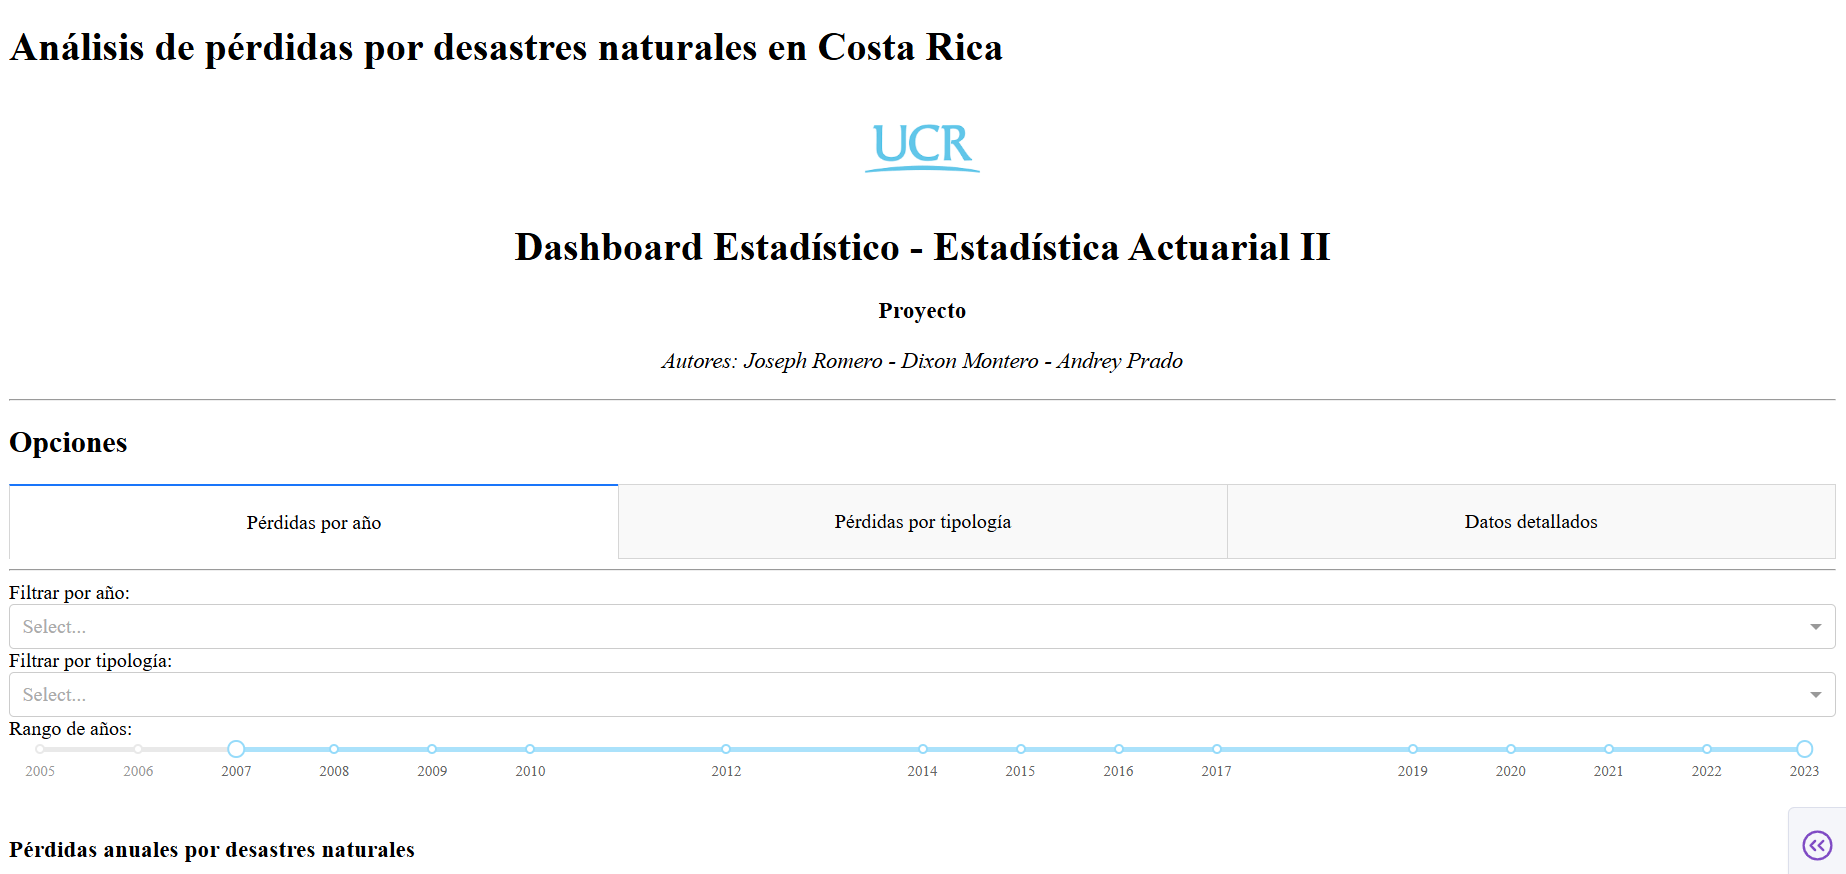
\includegraphics[width=0.9\textwidth]{fig/avance_dash_1/1.png}
\end{figure}
    \vspace{0.5cm}
\begin{figure}[htbp]
    \centering
    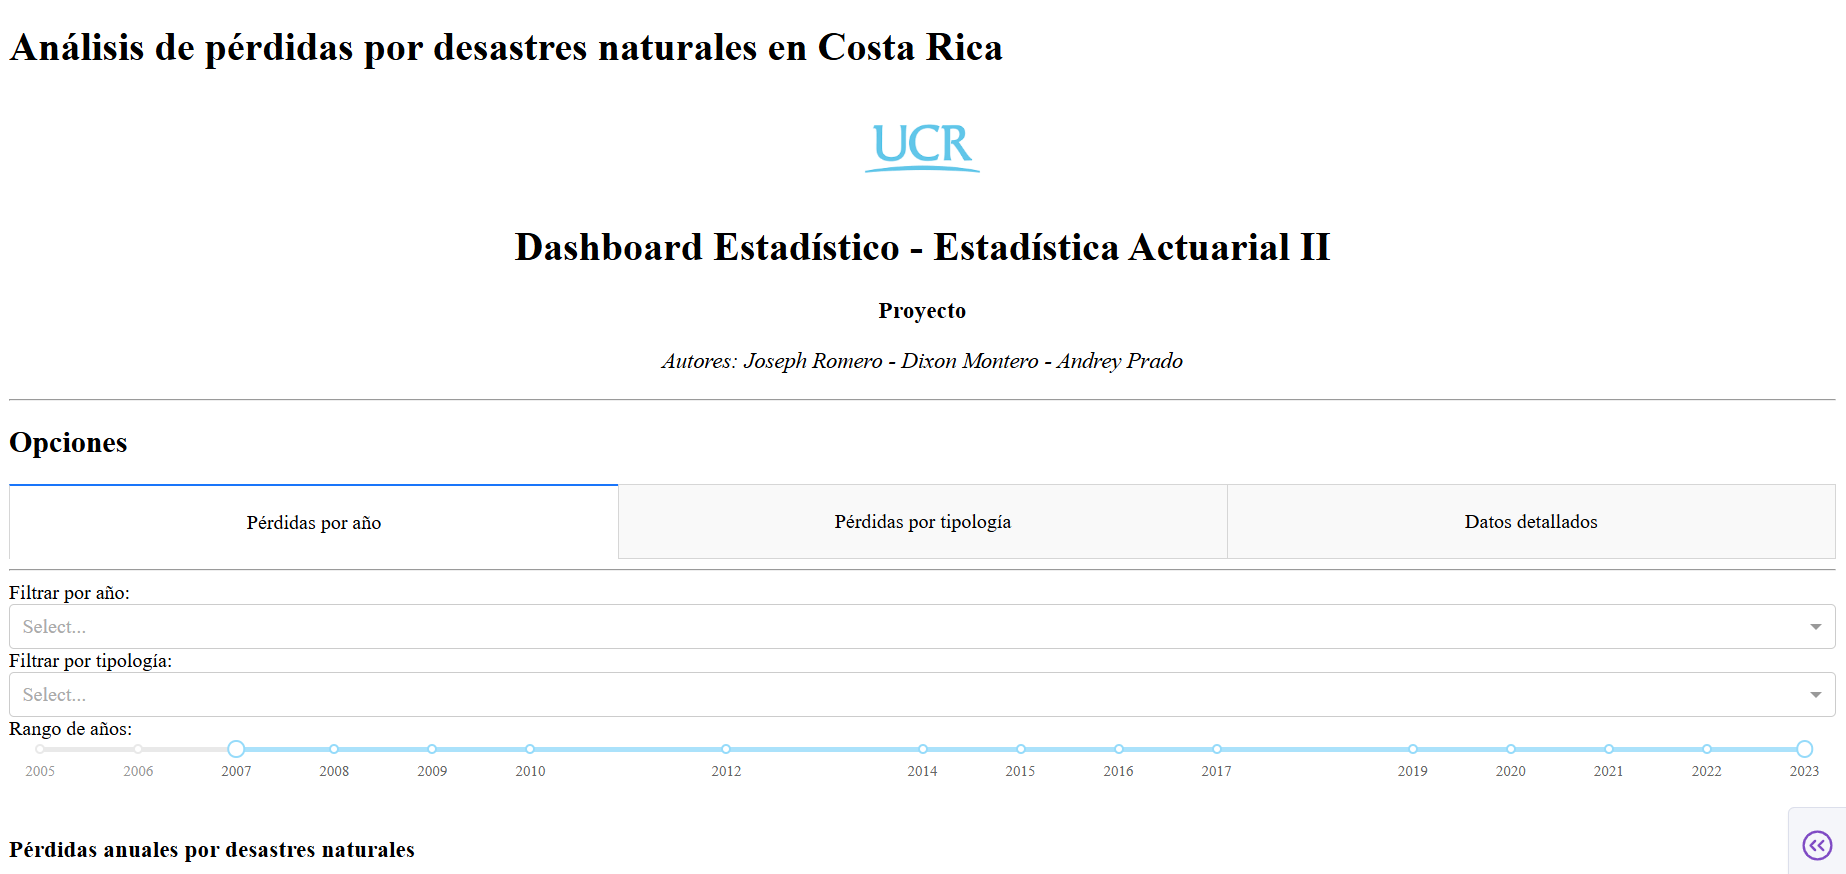
\includegraphics[width=0.9\textwidth]{fig/avance_dash_1/1.png}
\end{figure}
    \vspace{0.5cm}
\begin{figure}[htbp]
    \centering
    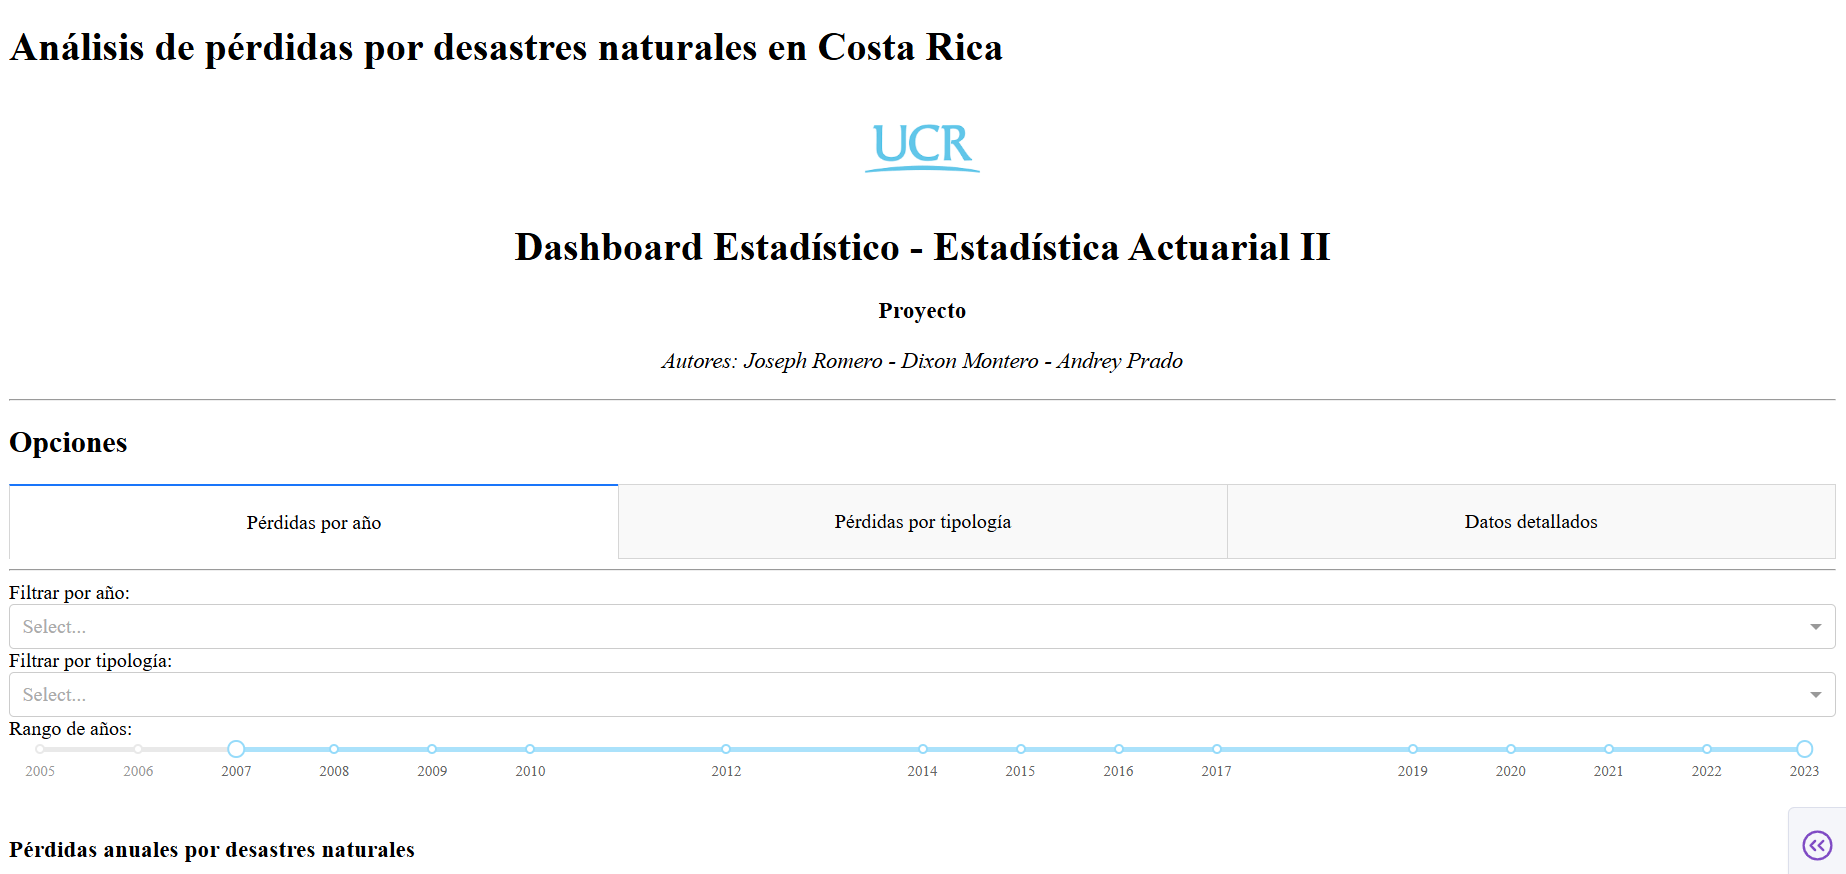
\includegraphics[width=0.9\textwidth]{fig/avance_dash_1/1.png}
\end{figure}
    \vspace{0.5cm}
\begin{figure}[htbp]
    \centering
    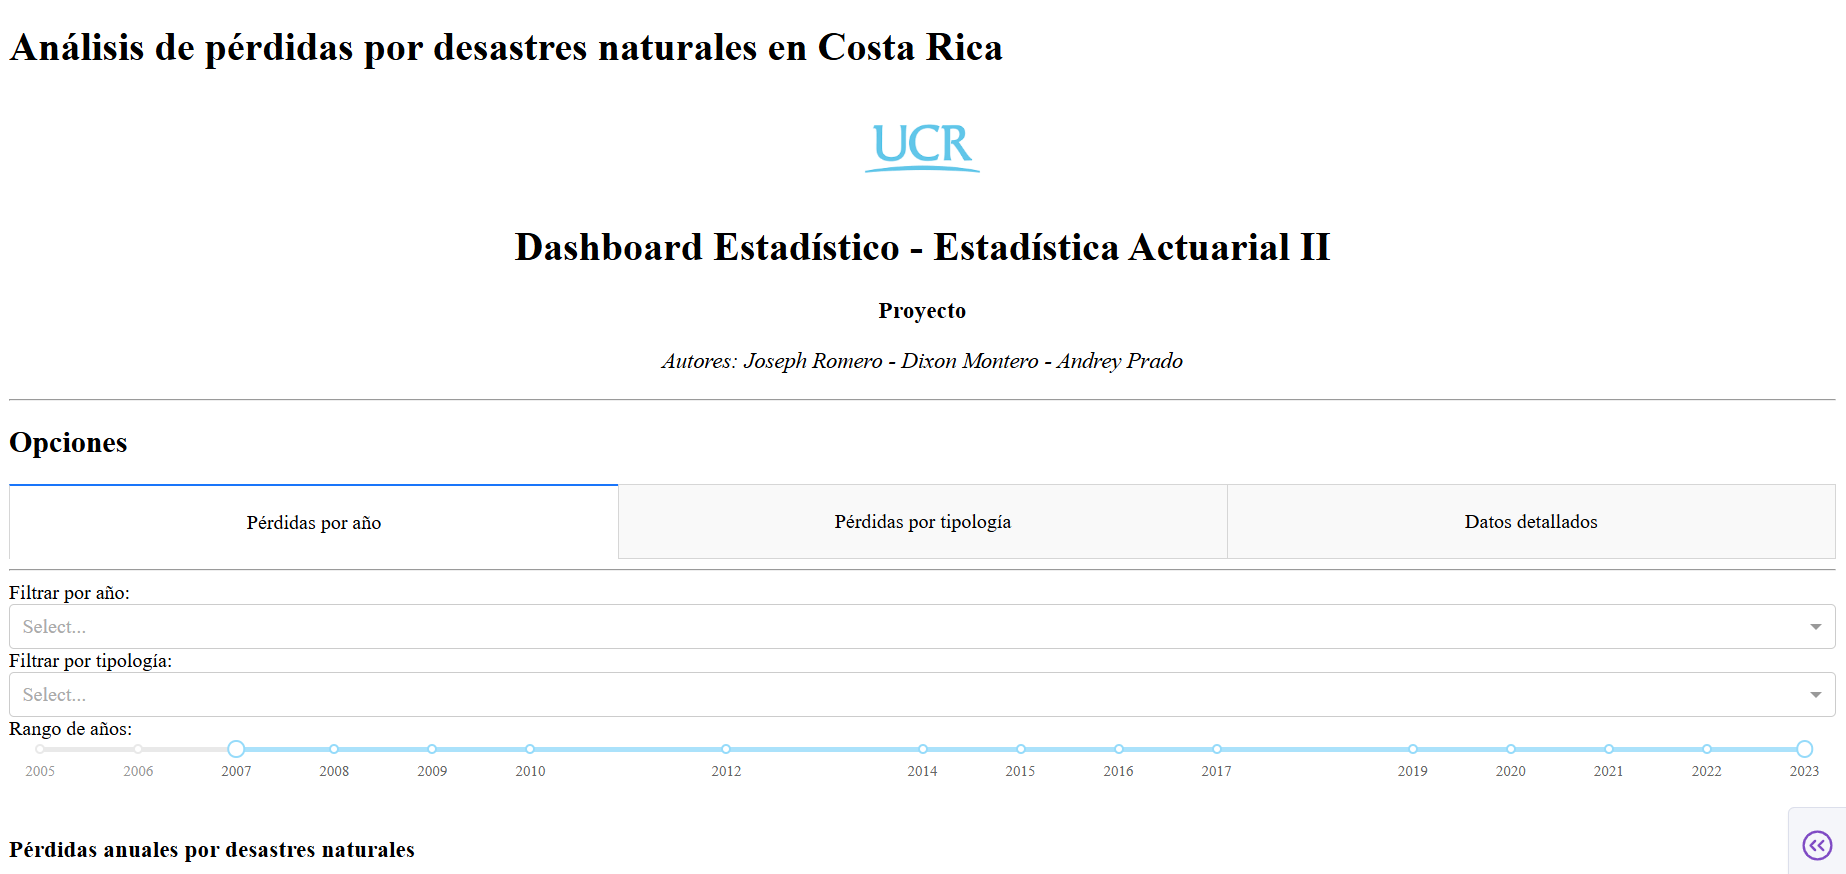
\includegraphics[width=0.9\textwidth]{fig/avance_dash_1/1.png}
\end{figure}
    \vspace{0.5cm}
\begin{figure}[htbp]
    \centering
    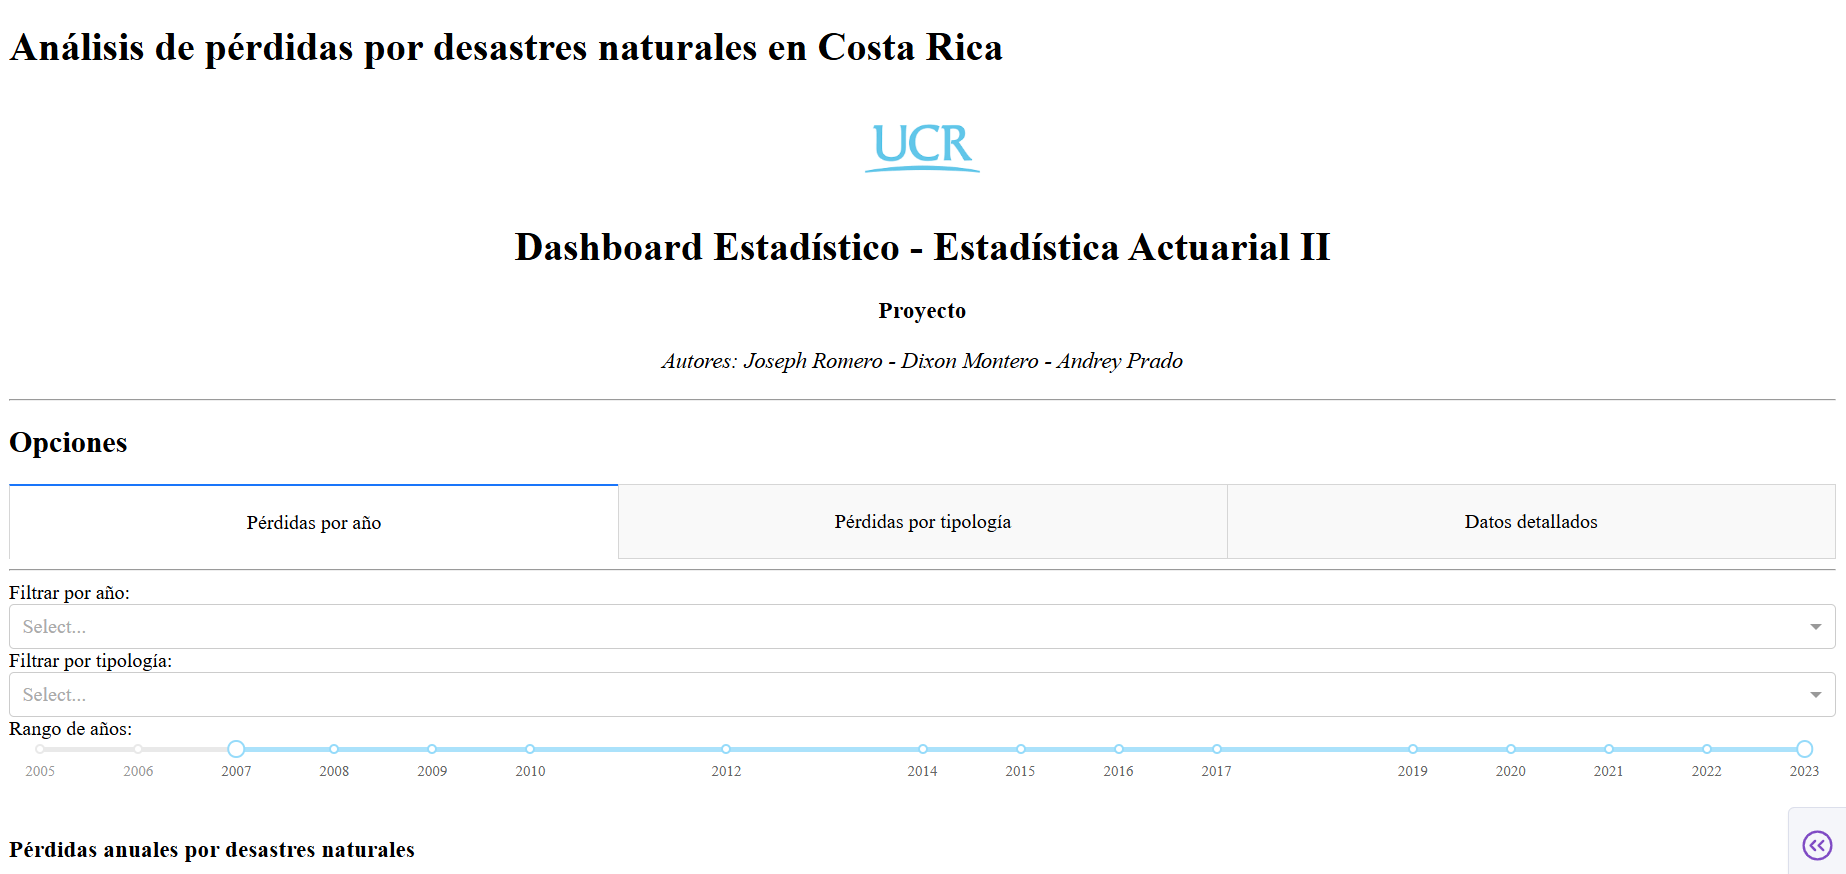
\includegraphics[width=0.9\textwidth]{fig/avance_dash_1/1.png}
\end{figure}

\newpage
\nocite{*}% Mostrar todas
\bibliography{referencias}
\end{document}
